%!TEX encoding = UTF-8 Unicode
% -*- coding: UTF-8; -*-
% vim: set fenc-utf-8

\chapter{Cas d'utilisations}
\label{s:cas_utilisation}

Ce chapitre présente les différents cas d'utilisation pour l'application VisuaLigue.
La figure \ref{fig:cas_utilisation_diag} résume les acteurs du systèmes et les cas d'utilisations.
La suite du chapitre décrie en détails les cas d'utilisations et s'attarde sur les plus importants.

\begin{figure}[htpb]
    \centering
    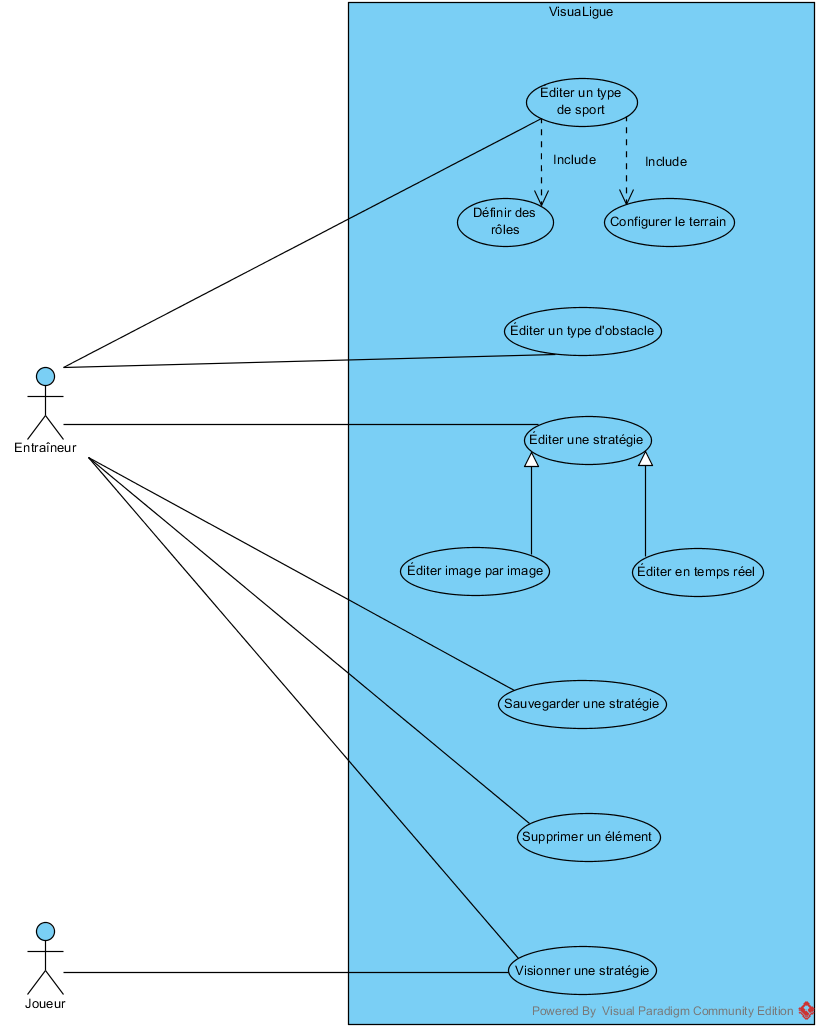
\includegraphics[scale=0.7]{fig/cas_utilisation_diag.png}
    \caption{Diagramme des cas d'utilisations}
    \label{fig:cas_utilisation_diag}
\end{figure}

\newpage



\section{Ajouter un type de sport}
\label{sec:ajouter_un_type_de_sport}

\subsection{Sc\'enario principal}
\label{sub:sc'enario_principal}

L'entra\^ineur cr\'ee un sport, le nomme.
Ensuite il ajoute les r\^oles du sport.
Finalement, il d\'efini un terrain en dessinant les lignes et en sp\'ecifiant les dimensions.

\subsection{Autres Situations}
\label{sub:autres_situations}
\begin{itemize}
    \item \textbf{Sport d\'ej\`a existant:} Si le sport existe d\'ej\`a dans l'application, un message d'avertissement appara\^it pour signaler que le sport existe d\'ej\`a.
    L'entraîneur peut d\'ecider d'effacer ce qui \'etait dans le sport existant, d'enregister son sport sous un autre nom, ou d'oublier le sport cr\'e\'e.
\end{itemize}


\section{Ajouter une strat\'egie}
\label{sec:ajouter_une_strat'egie}

\subsection{Pr\'erequis}
\label{sub:prerequis}

Le sport pour lequel l'entraîneur veut ajouter une stratégie doit exister dans l'application.

\subsection{Sc\'enario principal}
\label{sub:sc'enario_principal}

L'entra\^ineur veut ajouter une nouvelle strat\'egie.
Il lui assigne un identifiant et choisi un type de sport pour la strat\'egie.

\subsection{Autres situations}
\label{sub:autres_situations}
\begin{itemize}
    \item \textbf{Sport d\'ej\`a existant:} Si la stratégie existe d\'ej\`a dans l'application, un message d'avertissement appara\^it.
        L'entra\^ineur a alors le choix entre \'ecraser la strat\'egie existante ou d'annuler son ajout.
\end{itemize}



\section{\'Editer une stratégie}
\label{sec:ajouter_une_strategie}

\subsection{Sc\'enario principal}
\label{sub:sc'enario_principal}

L'entraîneur assigne les r\^oles aux diff\'erents joueurs.
Ensuite, il peut s\'electionner un joueur et tracer un mouvement ou interargir avec le projectile.
Pendant que le joueur est s\'electionn\'e, une simulation en temps r\'eel des mouvements pr\'ec\'edemment d\'efinies s'ex\'ecute.
L'entraîneur peut ensuite s\'electionner un autre joueur et dessiner une nouvelle action et la simulation recommence du d\'ebut.

\subsection{Autres situations}
\label{sub:autres_situations}

\begin{itemize}
    \item \textbf{Édition en mode image par image:} L'entraîneur édite la strat\'egie image par image ...
\end{itemize}



\section{Visualiser une stratégie}
\label{sec:visualiser_une_strategie}

\subsection{Pr\'erequis}
\label{sub:prerequis}
Il faut que la strat\'egie soit enregistr\'ee dans l'application pour que l'entraîneur puisse la visualiser.

\subsection{Sc\'enario principal}
\label{sub:sc'enario_principal}

L'entra\^ineur s\'electionne la strat\'egie \`a visualiser.
Il d\'ebute la visualisation et observe le d\'eroulement de la strat\'egie.
Il peut mettre fin \`a la visualisation \`a tout moment.



\section{Sauvegarder une stratégie}
\label{sec:exporter_une_strategie}

\subsection{Sc\'enario principal}
\label{sub:sc'enario_principal}

L'entra\^ineur a modifié une strat\'egie et la sauvegarde.
L'application enregistre les \'el\'ements de la strat\'egie.

\subsection{Autres situations}
\label{sub:autres_situations}

\begin{itemize}
    \item \textbf{Exportation dans un format image:} L'entra\^ineur souhaite plut\^ot exporter la strat\'egie dans un format de fichier.
        Il s\'electionne le format de fichier et le nom pour l'exportation.
        L'application convertie la strat\'egie en une image et l'enregistre dans un fichier avec le bon nom.
\end{itemize}



\section{Charger une strat\'egie}
\label{sec:charger_une_strat'egie}

L'entra\^ineur souhaite \'editer une strat\'egie d\'ej\`a existante.
Il s\'electionne la bonne strat\'egie puis la charge.
